\section{Vehicle Stop Frequency}
\label{sec:Results_Stops}

Vehicle Stop frequency is the natural kinematic counterpart to the mean speed metric discussed in Section~\vref{sec:Results_MeanSpeed}. A decrease in the platoon’s mean speed is expected to be accompanied by a rise in complete halts. Table~\vref{tab:StopFreq} and Figures~\vref{fig:StopFreq_2077} to \vref{fig:StopFreq_3462} therefore recapitulate the structure of the previous section, yet emphasise discrete stop events rather than continuous velocity.

\paragraph{Low to Intermediate Demand ($69$--$692~\unit{\veh\per\hour}$).}
For light and moderate traffic flows, both \ac{eco-glosa} and \ac{flow-glosa} effectively and monotonically decrease the stop frequency as the \ac{mpr} increases. This demonstrates a clear benefit of \ac{glosa} systems in sub-saturated conditions. At a demand of $138~\unit{\veh\per\hour}$ under the HBEFA4 model, the \ac{eco-glosa} controller reduces the stop rate from an initial $0.415$ to $0.04~\unit{\stops\per\veh}$ at $90\%$ \ac{mpr}, a reduction of over $90\%$. The \ac{flow-glosa} algorithm achieves a similarly robust reduction in stops across this demand range.

\paragraph{Emerging Congestion ($1385$--$2077~\unit{\veh\per\hour}$).}
As the system approaches its capacity limit, the ability of \ac{glosa} to smooth traffic flow and prevent stops becomes even more critical. At a demand of $2077~\unit{\veh\per\hour}$, which starts at $0.53~\unit{\stops\per\veh}$ in the Standard case, both controllers remain highly effective (Figure~\vref{fig:StopFreq_2077}). The \ac{flow-glosa} controller steadily reduces stops with increasing \ac{mpr}, completely eliminating them by $100\%$. The \ac{eco-glosa} controller also significantly reduces stops at high penetration, although it can exhibit minor instability at low \ac{mpr} levels as it adapts to the denser traffic. Nonetheless, both strategies demonstrate strong queue-suppression capabilities just below the congestion threshold.

\begin{figure}[htbp]
  \centering
  \begin{subfigure}[b]{0.98\textwidth}
    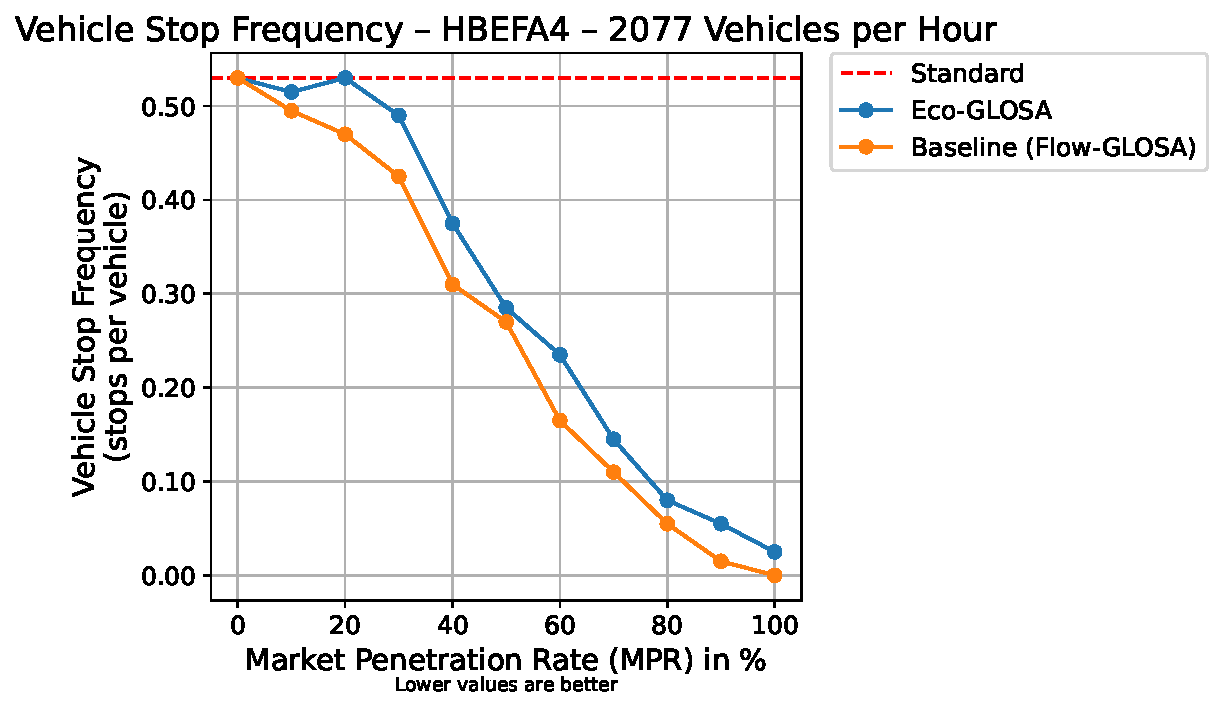
\includegraphics[width=\textwidth]{data/img/VehicleStopFrequency/VehicleStopFrequency_HBEFA4_Cars2077.pdf}
    \caption{Results under the HBEFA4 emission model.}
    \label{fig:StopFreq_2077_HBEFA4}
  \end{subfigure}
  \begin{subfigure}[b]{0.98\textwidth}
    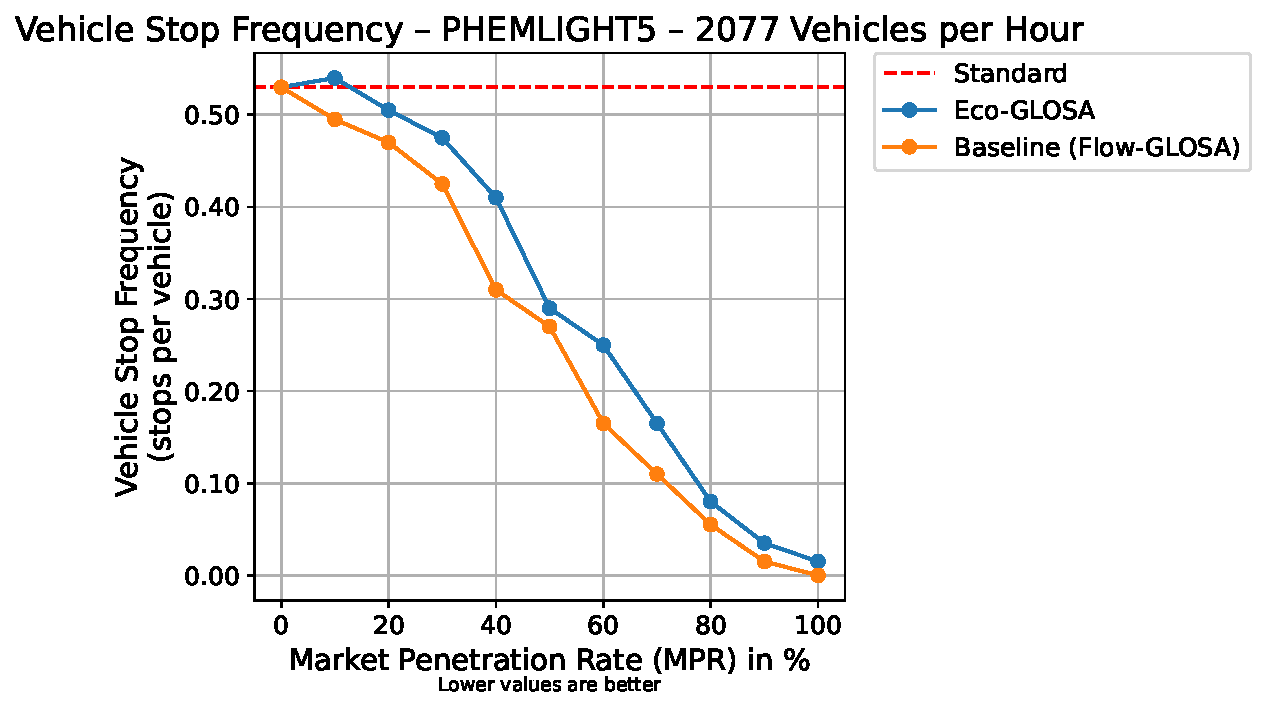
\includegraphics[width=\textwidth]{data/img/VehicleStopFrequency/VehicleStopFrequency_PHEMLIGHT5_Cars2077.pdf}
    \caption{Results under the PHEMlight5 emission model.}
    \label{fig:StopFreq_2077_PHEM}
  \end{subfigure}
  \caption[Vehicle stop frequency vs. \ac{mpr} at $2077~\unit{\veh\per\hour}$]{Vehicle stop frequency versus \ac{mpr} at an incipient congestion level of $2077~\unit{\veh\per\hour}$. The plots compare the Standard, \ac{eco-glosa}, and \ac{flow-glosa} controllers.}
  \label{fig:StopFreq_2077}
\end{figure}

\paragraph{High Demand ($2769~\unit{\veh\per\hour}$).}
This demand level reveals a critical performance divergence (Figure~\vref{fig:StopFreq_2769}). The \ac{flow-glosa} controller remains robust, maintaining a low stop frequency that declines smoothly as \ac{mpr} increases. In contrast, \ac{eco-glosa} becomes highly unstable. Under the PHEMlight5 model, its stop frequency increases sharply from the Standard value of $0.68~\unit{\stops\per\veh}$ to over $11.5~\unit{\stops\per\veh}$ at $90\%$ \ac{mpr}. The HBEFA4 model exhibits different volatility, with stop frequency oscillating and peaking at $8.02~\unit{\stops\per\veh}$ at $60\%$ \ac{mpr}. This behaviour highlights the risk of \ac{eco-glosa} actively inducing stop-and-go waves at the verge of congestion.

\begin{figure}[htbp]
  \centering
  \begin{subfigure}[b]{0.98\textwidth}
    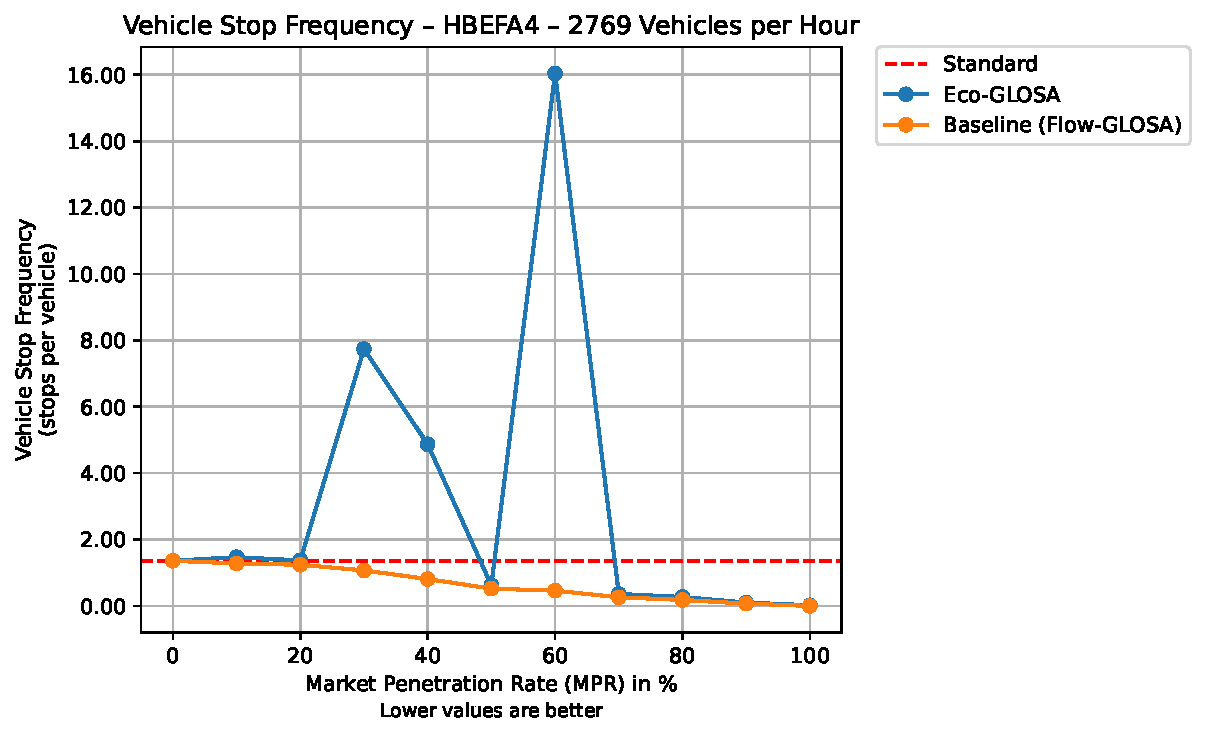
\includegraphics[width=\textwidth]{data/img/VehicleStopFrequency/VehicleStopFrequency_HBEFA4_Cars2769.pdf}
    \caption{Performance with the HBEFA4 emission model.}
    \label{fig:StopFreq_2769_HBEFA4}
  \end{subfigure}
  \begin{subfigure}[b]{0.98\textwidth}
    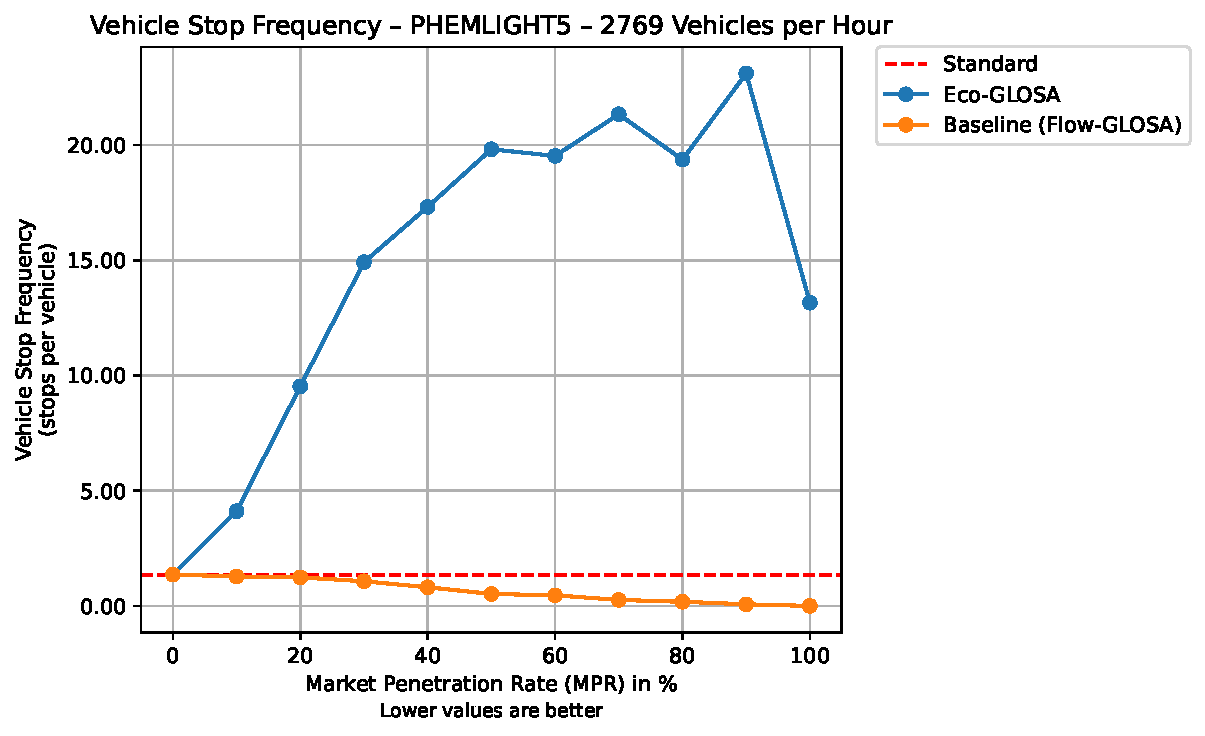
\includegraphics[width=\textwidth]{data/img/VehicleStopFrequency/VehicleStopFrequency_PHEMLIGHT5_Cars2769.pdf}
    \caption{Performance with the PHEMlight5 emission model.}
    \label{fig:StopFreq_2769_PHEM}
  \end{subfigure}
  \caption[Vehicle stop frequency vs. \ac{mpr} at $2769~\unit{\veh\per\hour}$]{Vehicle stop frequency versus \ac{mpr} at the jam threshold of $2769~\unit{\veh\per\hour}$. The plots illustrate the significant performance divergence of the two control strategies.}
  \label{fig:StopFreq_2769}
\end{figure}

\paragraph{Saturated Regime ($3462~\unit{\veh\per\hour}$).}
In the fully saturated regime, the Standard scenario is already gridlocked with a high stop frequency of $9.42~\unit{\stops\per\veh}$ (Figure~\vref{fig:StopFreq_3462}). Under these conditions, the \ac{eco-glosa} controller fails to improve conditions and instead exacerbates congestion, with its stop frequency increasing to over $17~\unit{\stops\per\veh}$ (HBEFA4) and $19~\unit{\stops\per\veh}$ (PHEMlight5). In the opposite direction, the \ac{flow-glosa} controller demonstrates a remarkable ability to prevent gridlock. Its effectiveness becomes apparent as penetration increases, with the stop frequency dropping sharply beyond $50\%$ \ac{mpr}. At full penetration, stops are reduced to near-zero levels ($0.005~\unit{\stops\per\veh}$). This profound reduction, supported by the sustained high average speeds shown in Figure~\vref{fig:MeanSpeed_3462}, confirms that a flow-optimised strategy successfully maintains free-flow conditions and prevents the onset of severe traffic jams even under saturated demand.

\begin{figure}[htbp]
  \centering
  \begin{subfigure}[b]{0.98\textwidth}
    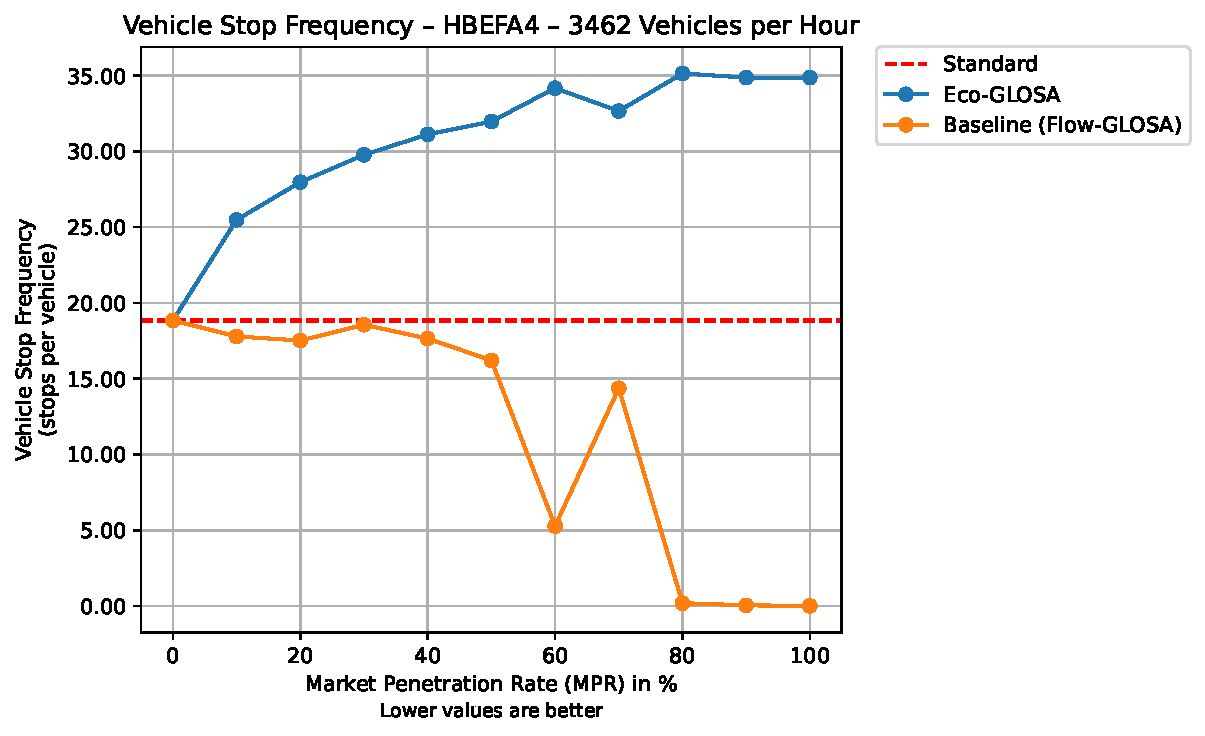
\includegraphics[width=\textwidth]{data/img/VehicleStopFrequency/VehicleStopFrequency_HBEFA4_Cars3462.pdf}
    \caption{Simulation results using the HBEFA4 model.}
    \label{fig:StopFreq_3462_HBEFA4}
  \end{subfigure}
  \begin{subfigure}[b]{0.98\textwidth}
    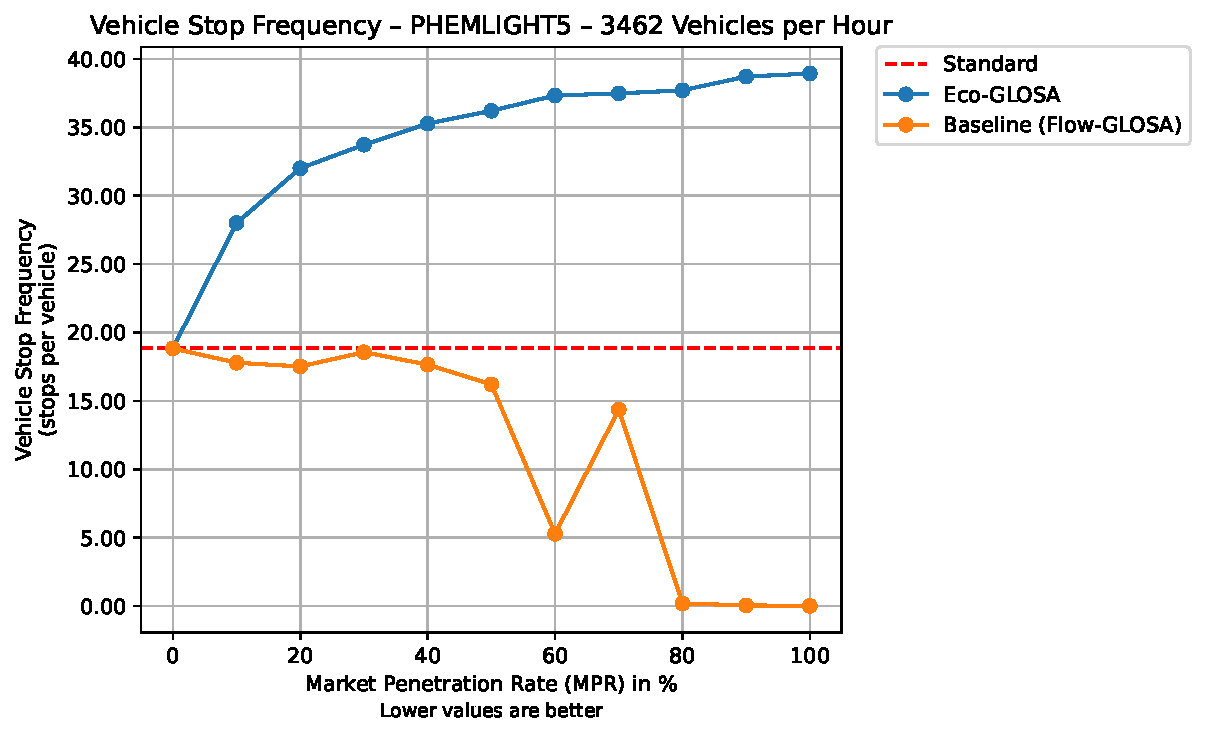
\includegraphics[width=\textwidth]{data/img/VehicleStopFrequency/VehicleStopFrequency_PHEMLIGHT5_Cars3462.pdf}
    \caption{Simulation results using the PHEMlight5 model.}
    \label{fig:StopFreq_3462_PHEM}
  \end{subfigure}
  \caption[Vehicle stop frequency vs. \ac{mpr} at $3462~\unit{\veh\per\hour}$]{Vehicle stop frequency as a function of \ac{mpr} in the fully saturated regime of $3462~\unit{\veh\per\hour}$. The outcomes for the Standard, \ac{eco-glosa}, and \ac{flow-glosa} controllers are shown.}
  \label{fig:StopFreq_3462}
\end{figure}

\paragraph{Implications.}
The stop frequency results reveal a significant performance inversion for the \ac{eco-glosa} controller. While it is highly effective at reducing stops in low to moderate demand, its behaviour becomes inconsistent and counterproductive as the system approaches capacity, actively increasing stops and inducing traffic instability. This creates a substantial operational risk, where a controller intended to improve efficiency instead causes network instability. The choice of emission model further complicates its performance, with the transient-sensitive PHEMlight5 model consistently triggering this failure at lower penetration rates than HBEFA4. Conversely, the \ac{flow-glosa} algorithm proves to be a robust strategy across all demand scenarios. Its consistent ability to suppress and prevent vehicle stops, particularly under high and saturated demand, underscores its value not just for optimising flow but for ensuring network stability.

\paragraph{Key Takeaways.}
\begin{enumerate}
    \item \textbf{Low Demand Performance:} In light to moderate demand scenarios ($69$--$1385~\unit{\veh\per\hour}$), both \ac{eco-glosa} and \ac{flow-glosa} are highly effective, significantly reducing vehicle stop frequency as their market penetration increases.
    \item \textbf{Performance Inversion:} \ac{eco-glosa} exhibits a critical performance inversion. Its benefits in low-demand scenarios are reversed at high demands ($ \geq 2769~\unit{\veh\per\hour}$), where it becomes unstable and significantly increases stop frequency compared to the uncontrolled Standard.
    \item \textbf{Robustness of \ac{flow-glosa}:} The \ac{flow-glosa} controller is robust across all tested demand levels, consistently maintaining or reducing stop frequency.
    \item \textbf{Gridlock Prevention:} In fully saturated conditions ($3462~\unit{\veh\per\hour}$), where the Standard scenario is gridlocked, \ac{flow-glosa} is capable of preventing this breakdown. At high penetration rates, it drives stop counts to near-zero, thereby maintaining free-flow conditions.
\end{enumerate}

\begin{table}[htb]
  \centering
  \caption[Vehicle stop frequency for all traffic volumes and \ac{mpr} values]{Vehicle stop frequency, measured in $\unit{\stops\per\veh}$, tabulated for all traffic volumes and \ac{mpr} values. Data is provided for the Standard, \ac{flow-glosa}, and \ac{eco-glosa} controllers under both the HBEFA4 and PHEMlight5 emission models.}
  \label{tab:StopFreq}
  \resizebox{\textwidth}{!}{%
  \begin{tabular}{r l l r *{10}{r}}
    \toprule
    Vehicles & Algorithm & Fuel Model & \textbf{0\% (Standard)} & 10\% & 20\% & 30\% & 40\% & 50\% & 60\% & 70\% & 80\% & 90\% & 100\%\\
    \midrule
    69  & \ac{eco-glosa} & HBEFA4 & \textbf{0.38} & 0.28 & 0.36 & 0.28 & 0.245 & 0.27 & 0.215 & 0.11 & 0.14 & 0.055 & 0\\
    69  & Baseline (\ac{flow-glosa}) & HBEFA4 & \textbf{0.38} & 0.28 & 0.39 & 0.305 & 0.245 & 0.27 & 0.245 & 0.11 & 0.14 & 0.085 & 0\\
    69  & \ac{eco-glosa} & PHEMLIGHT5 & \textbf{0.38} & 0.28 & 0.36 & 0.25 & 0.245 & 0.27 & 0.215 & 0.11 & 0.14 & 0.055 & 0\\
    69  & Baseline (\ac{flow-glosa}) & PHEMLIGHT5 & \textbf{0.38} & 0.28 & 0.39 & 0.305 & 0.245 & 0.27 & 0.245 & 0.11 & 0.14 & 0.085 & 0\\
    \midrule
    138 & \ac{eco-glosa} & HBEFA4 & \textbf{0.415} & 0.32 & 0.32 & 0.295 & 0.185 & 0.135 & 0.135 & 0.095 & 0.065 & 0.04 & 0\\
    138 & Baseline (\ac{flow-glosa}) & HBEFA4 & \textbf{0.415} & 0.305 & 0.31 & 0.295 & 0.185 & 0.16 & 0.12 & 0.08 & 0.08 & 0.025 & 0\\
    138 & \ac{eco-glosa} & PHEMLIGHT5 & \textbf{0.415} & 0.335 & 0.28 & 0.295 & 0.185 & 0.145 & 0.08 & 0.095 & 0.065 & 0.04 & 0\\
    138 & Baseline (\ac{flow-glosa}) & PHEMLIGHT5 & \textbf{0.415} & 0.305 & 0.31 & 0.295 & 0.185 & 0.16 & 0.12 & 0.08 & 0.08 & 0.025 & 0\\
    \midrule
    346 & \ac{eco-glosa} & HBEFA4 & \textbf{0.38} & 0.34 & 0.325 & 0.255 & 0.235 & 0.19 & 0.14 & 0.135 & 0.095 & 0.04 & 0.005\\
    346 & Baseline (\ac{flow-glosa}) & HBEFA4 & \textbf{0.38} & 0.345 & 0.32 & 0.245 & 0.22 & 0.18 & 0.12 & 0.135 & 0.075 & 0.03 & 0\\
    346 & \ac{eco-glosa} & PHEMLIGHT5 & \textbf{0.38} & 0.325 & 0.365 & 0.28 & 0.255 & 0.175 & 0.155 & 0.135 & 0.085 & 0.035 & 0.015\\
    346 & Baseline (\ac{flow-glosa}) & PHEMLIGHT5 & \textbf{0.38} & 0.345 & 0.32 & 0.245 & 0.22 & 0.18 & 0.12 & 0.135 & 0.075 & 0.03 & 0\\
    \midrule
    692 & \ac{eco-glosa} & HBEFA4 & \textbf{0.395} & 0.39 & 0.31 & 0.27 & 0.225 & 0.21 & 0.115 & 0.13 & 0.08 & 0.03 & 0.005\\
    692 & Baseline (\ac{flow-glosa}) & HBEFA4 & \textbf{0.395} & 0.35 & 0.315 & 0.265 & 0.225 & 0.185 & 0.115 & 0.11 & 0.065 & 0.025 & 0.005\\
    692 & \ac{eco-glosa} & PHEMLIGHT5 & \textbf{0.395} & 0.345 & 0.33 & 0.3 & 0.25 & 0.205 & 0.145 & 0.125 & 0.1 & 0.025 & 0.005\\
    692 & Baseline (\ac{flow-glosa}) & PHEMLIGHT5 & \textbf{0.395} & 0.35 & 0.315 & 0.265 & 0.225 & 0.185 & 0.115 & 0.11 & 0.065 & 0.025 & 0.005\\
    \midrule
    1385 & \ac{eco-glosa} & HBEFA4 & \textbf{0.455} & 0.45 & 0.41 & 0.345 & 0.29 & 0.23 & 0.205 & 0.125 & 0.095 & 0.05 & 0.01\\
    1385 & Baseline (\ac{flow-glosa}) & HBEFA4 & \textbf{0.455} & 0.42 & 0.395 & 0.35 & 0.275 & 0.2 & 0.155 & 0.105 & 0.065 & 0.04 & 0\\
    1385 & \ac{eco-glosa} & PHEMLIGHT5 & \textbf{0.455} & 0.445 & 0.405 & 0.375 & 0.285 & 0.215 & 0.215 & 0.11 & 0.11 & 0.045 & 0.025\\
    1385 & Baseline (\ac{flow-glosa}) & PHEMLIGHT5 & \textbf{0.455} & 0.42 & 0.395 & 0.35 & 0.275 & 0.2 & 0.155 & 0.105 & 0.065 & 0.04 & 0\\
    \midrule
    2077 & \ac{eco-glosa} & HBEFA4 & \textbf{0.53} & 0.515 & 0.53 & 0.49 & 0.375 & 0.285 & 0.235 & 0.145 & 0.08 & 0.055 & 0.025\\
    2077 & Baseline (\ac{flow-glosa}) & HBEFA4 & \textbf{0.53} & 0.495 & 0.47 & 0.425 & 0.31 & 0.27 & 0.165 & 0.11 & 0.055 & 0.015 & 0\\
    2077 & \ac{eco-glosa} & PHEMLIGHT5 & \textbf{0.53} & 0.54 & 0.505 & 0.475 & 0.41 & 0.29 & 0.25 & 0.165 & 0.08 & 0.035 & 0.015\\
    2077 & Baseline (\ac{flow-glosa}) & PHEMLIGHT5 & \textbf{0.53} & 0.495 & 0.47 & 0.425 & 0.31 & 0.27 & 0.165 & 0.11 & 0.055 & 0.015 & 0\\
    \midrule
    \textbf{2769} & \textbf{\ac{eco-glosa}} & \textbf{HBEFA4} & \textbf{0.68} & \textbf{0.735} & \textbf{0.685} & \textbf{3.87} & \textbf{2.435} & \textbf{0.31} & \textbf{8.02} & \textbf{0.18} & \textbf{0.135} & \textbf{0.05} & \textbf{0.01}\\
    2769 & Baseline (\ac{flow-glosa}) & HBEFA4 & \textbf{0.68} & 0.64 & 0.62 & 0.535 & 0.405 & 0.26 & 0.23 & 0.13 & 0.09 & 0.035 & 0\\
    \textbf{2769} & \textbf{\ac{eco-glosa}} & \textbf{PHEMLIGHT5} & \textbf{0.68} & \textbf{2.055} & \textbf{4.765} & \textbf{7.46} & \textbf{8.66} & \textbf{9.91} & \textbf{9.765} & \textbf{10.67} & \textbf{9.685} & \textbf{11.555} & \textbf{6.58}\\
    2769 & Baseline (\ac{flow-glosa}) & PHEMLIGHT5 & \textbf{0.68} & 0.64 & 0.62 & 0.535 & 0.405 & 0.26 & 0.23 & 0.13 & 0.09 & 0.035 & 0\\
    \midrule
    \textbf{3462} & \textbf{\ac{eco-glosa}} & \textbf{HBEFA4} & \textbf{9.42} & \textbf{12.74} & \textbf{13.985} & \textbf{14.885} & \textbf{15.56} & \textbf{15.985} & \textbf{17.085} & \textbf{16.33} & \textbf{17.57} & \textbf{17.435} & \textbf{17.435}\\
    3462 & Baseline (\ac{flow-glosa}) & HBEFA4 & \textbf{9.42} & 8.895 & 8.76 & 9.28 & 8.825 & 8.105 & 2.64 & 7.185 & \textbf{0.095} & \textbf{0.025} & \textbf{0.005}\\
    \textbf{3462} & \textbf{\ac{eco-glosa}} & \textbf{PHEMLIGHT5} & \textbf{9.42} & \textbf{14.005} & \textbf{16.005} & \textbf{16.865} & \textbf{17.635} & \textbf{18.105} & \textbf{18.665} & \textbf{18.74} & \textbf{18.855} & \textbf{19.355} & \textbf{19.47}\\
    3462 & Baseline (\ac{flow-glosa}) & PHEMLIGHT5 & \textbf{9.42} & 8.895 & 8.76 & 9.28 & 8.825 & 8.105 & 2.64 & 7.185 & \textbf{0.095} & \textbf{0.025} & \textbf{0.005}\\
    \bottomrule
  \end{tabular}}
\end{table}